\section{Analysis}
\label{sec:results}

We organize the analysis around four questions, namely which benchmarks provide signal on small multilingual models (\ref{subsec:exp-da}), which SNR definition best predicts decision accuracy (\ref{subsec:exp-snr-da}), whether the resulting ranking generalizes across seeds and model suites (\ref{subsec:exp-generalization}), and whether benchmark subsets and design choices can improve reliability (\ref{subsec:exp-benchmark-design}).

\subsection{Calculation of Decision Accuracy}
\label{subsec:exp-da}

\textbf{Checkpoint selection.} For each custom and open-source model, we evaluate 10 evenly spaced checkpoints across training and 5 additional checkpoints in the final 10\% of training FLOPS. This schedule captures both the long-range trajectory and the late-training variation.

\textbf{The above-random gate.} Before computing DA or SNR, we filter (benchmark, size) cells whose mean score does not exceed the random baseline by at least 5 points. Figure~\ref{fig:gate} illustrates the two regimes. Of 118 benchmarks\footnote{Since we analyze results by language, we consider each language subset as a different benchmark (i.e. \texttt{hellaswag\_es} and \texttt{hellaswag\_hi} are two different benchmarks.}, only 44 clear chance at one or more custom model sizes, and 74 are at chance everywhere. The failures are almost entirely an answer-count effect, since four-option translated knowledge tasks sit at chance across all custom sizes while two-option tasks clear the gate. Notably, the three benchmarks that separate the data mixtures most are exactly the ones the gate removes. Their apparent signal is variation around chance, not capability. This shows that raw score separation cannot guide benchmark selection on its own.

\begin{figure}[t]
\centering
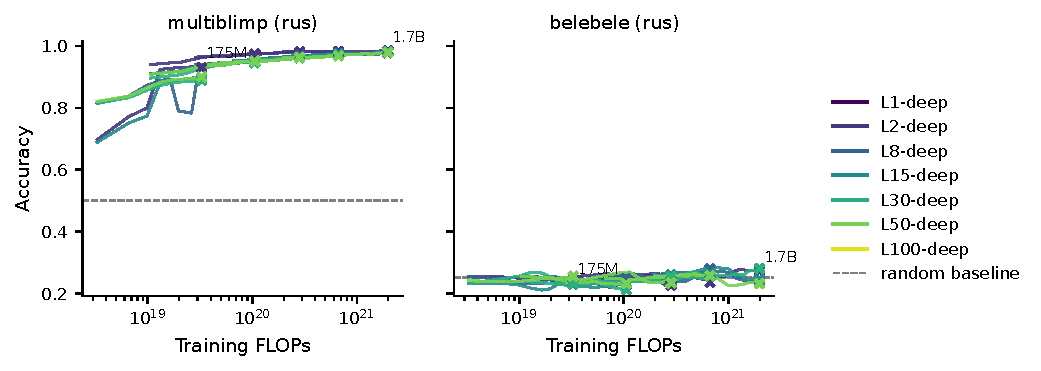
\includegraphics[width=0.7\textwidth]{figures/fig1_gate.pdf}
\caption{The above-random gate. Accuracy against training compute for the three data mixtures (colored curves) with final checkpoints marked. Left, a benchmark that clears the gate (\texttt{multiblimp}) shows scores well above the random baseline (dashed line) and consistent mixture separation.
Right, a gated benchmark (\texttt{belebele}) fluctuates around its baseline, so any apparent separation between mixtures is noise. A (benchmark, size) cell is kept iff its mean score exceeds the baseline by 5 points.}
\label{fig:gate}
\end{figure}

\textbf{Extension with external models.} Many tasks are at chance for the custom models, which are trained on 200 languages with only 100B tokens and at most 1B parameters. We therefore extend the analysis with 68 external models from 270M to 70B parameters (Appendix Table~\ref{tab:external}).
External sizes pool into buckets so that each bucket holds at least two models, and buckets contribute to signal and decision accuracy while singleton sizes only appear on the accuracy curves. With capable models in the pool, additional benchmarks clear the gate and enter the analysis.

% TODO: Figure or table showing acc vs flops and or top DA benchmarks, per DA type, and per language

\textbf{Per-language reliability at small scale.} Figure~\ref{fig:reliability-map} shows the full benchmark-by-language map for the above-random benchmarks on the small pretrained models. MultiBLiMP is the most reliable benchmark in six of eleven languages, with decision accuracy between 0.79 and 0.87, which matches the expectation that grammatical acceptability emerges early and therefore discriminates small models. Swahili retains no above-random benchmark on the custom models, so no reliable small-scale decision can be made for it at this scale. This confirms that benchmark reliability is language dependent and motivates the per-language reliability map as the practical output of the framework.

\textbf{Per-language reliability at 32B.} 
Table~\ref{tab:reliability-map} reports,
for each language, the benchmark whose small-model rankings best transfer to large models on the external suite. For each benchmark and language we average decision accuracy over all small-to-large size pairs, with small models up to 1.7B and large models from 7B to 32B parameters. Human-translated narrative and commonsense tasks dominate. XStoryCloze is the most transferable benchmark in four languages and close behind in three more, with decision accuracy up to 0.99, while machine-translated knowledge tasks rarely lead. The most reliable benchmark differs by language, and for Swahili no benchmark exceeds 0.57, barely above a random decision. This confirms that benchmark reliability is language dependent and that a single universal benchmark choice leaves some languages effectively unmeasured.

\begin{figure}[t]
\centering
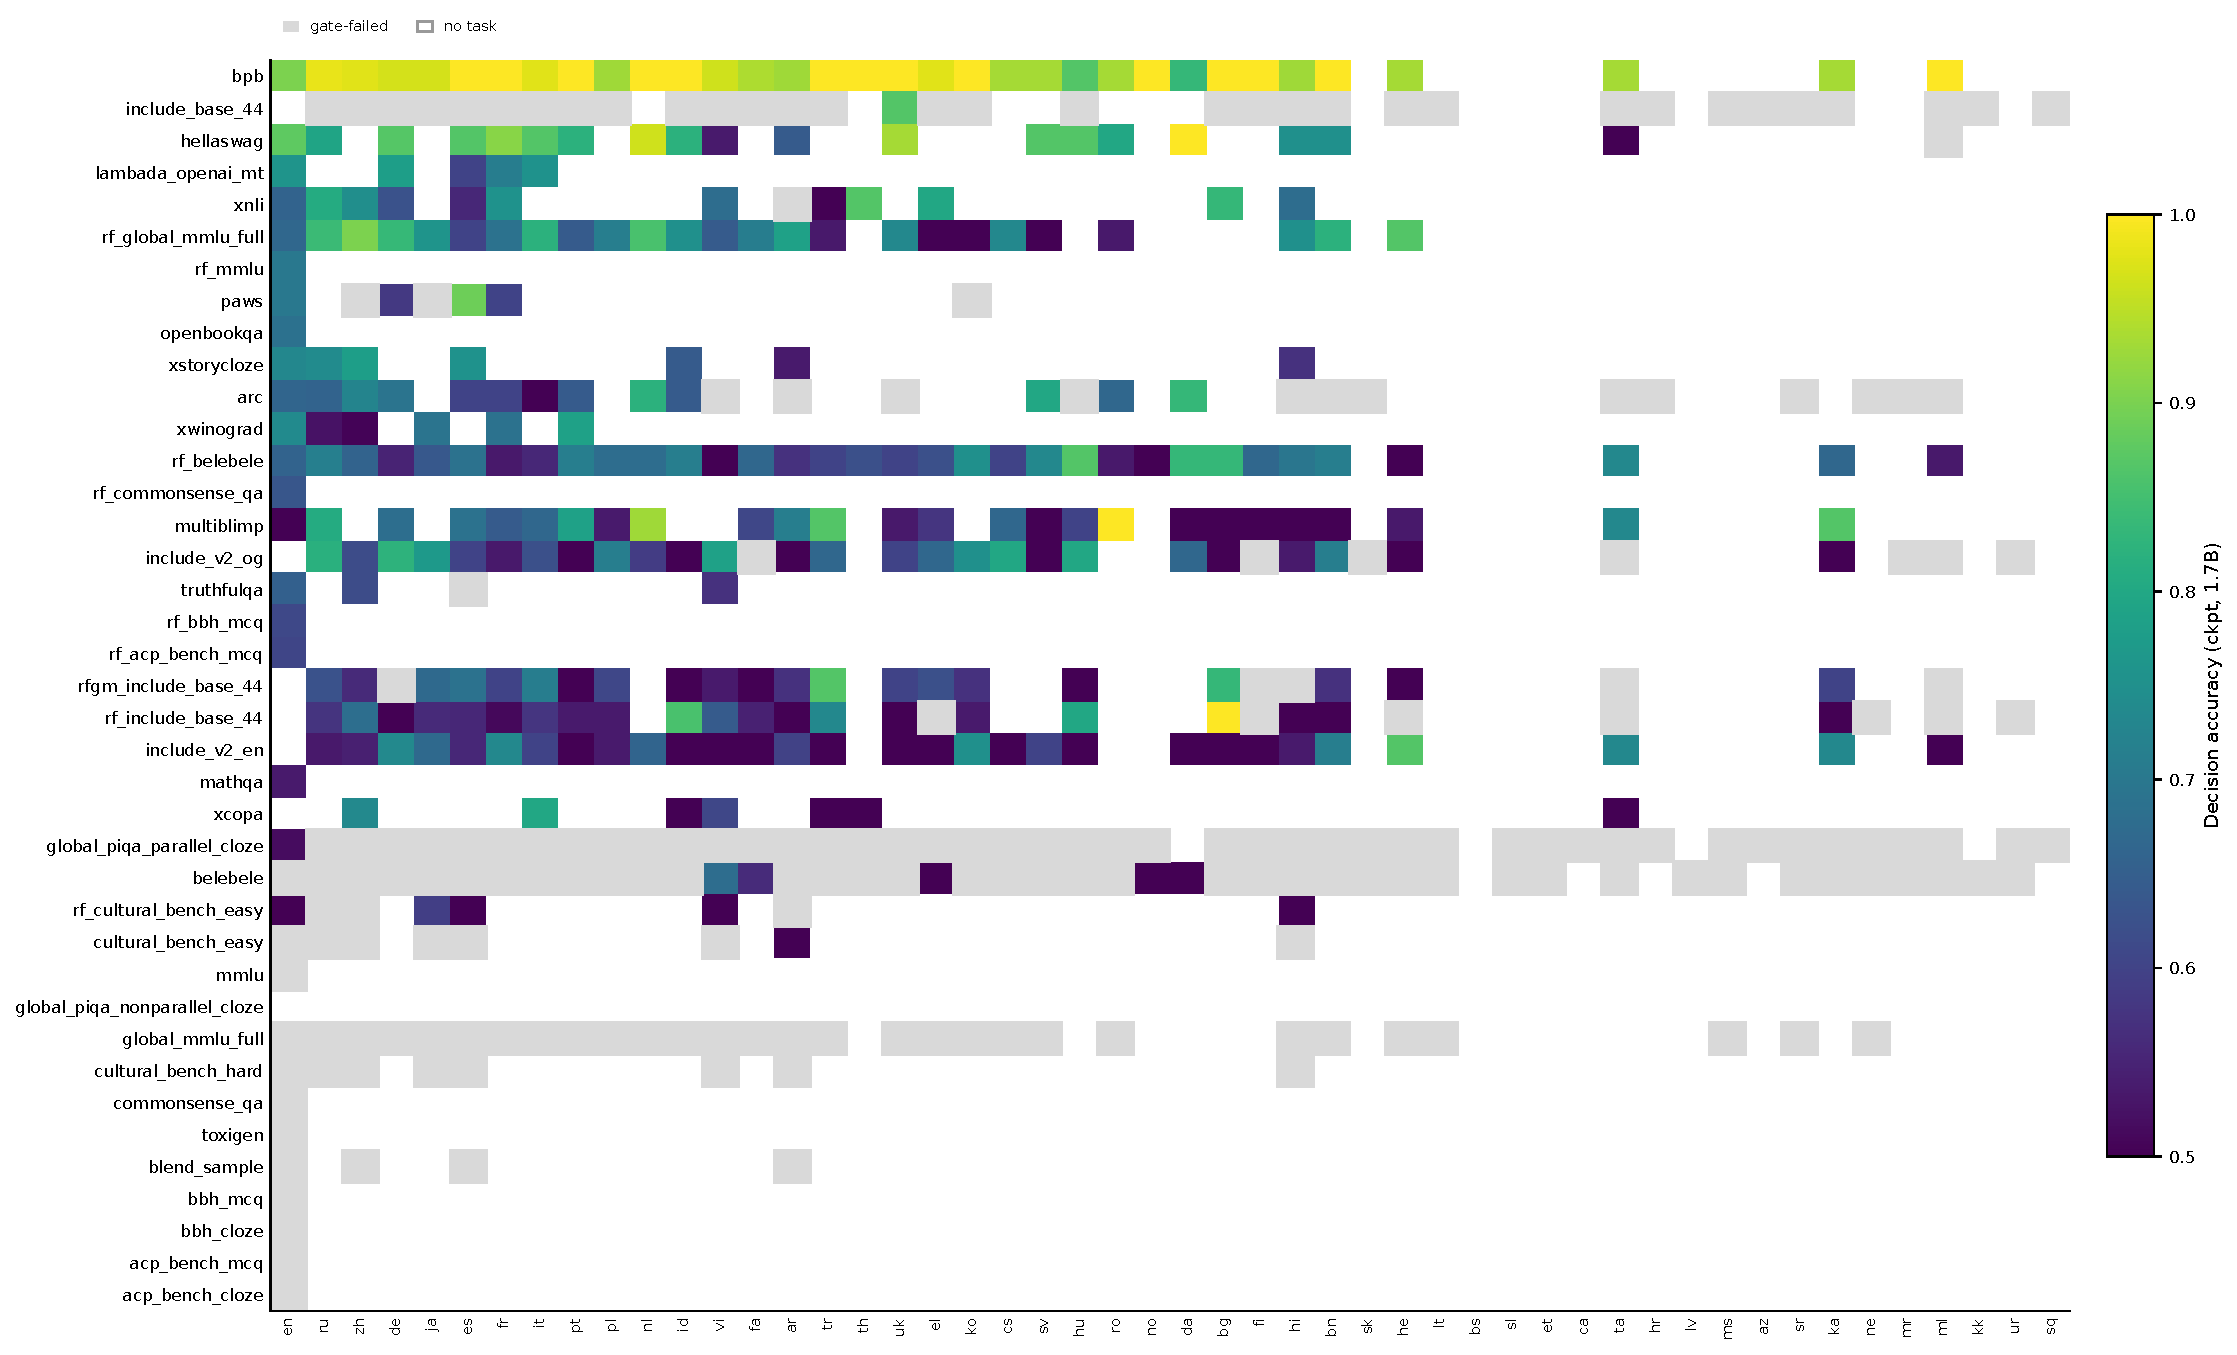
\includegraphics[width=0.7\textwidth]{figures/fig3_reliability_map.pdf}
\caption{Benchmark reliability map. Decision accuracy by checkpoint at the 1B target for every benchmark family and language. Grey cells fail the above-random gate. Practitioners can read off which benchmarks support small-scale decisions for their target languages.}
\label{fig:reliability-map}
\end{figure}

\begin{table}[t]
\centering
\small
\caption{Per-language reliability map on the external suite (68 open-source models, 270M to 70B). For each language, the benchmark with the highest decision accuracy averaged over the nine small-to-large size pairs (small $\leq$ 1.7B, large 7B to 32B). DA is the fraction of model pairs whose small-scale ranking holds at large scale.}
\label{tab:reliability-map}
\begin{tabular}{llclc}
\toprule
Lang & Top benchmark & DA & Runner-up & DA \\
\midrule
en & \texttt{xwinograd}         & 0.81 & \texttt{xstorycloze} & 0.76 \\
es & \texttt{hellaswag}         & 0.97 & \texttt{xstorycloze} & 0.76 \\
ru & \texttt{xstorycloze}       & 0.99 & \texttt{hellaswag}   & 0.95 \\
hi & \texttt{xstorycloze}       & 0.78 & \texttt{multiblimp}  & 0.74 \\
zh & \texttt{xstorycloze}       & 0.97 & \texttt{xcopa}       & 0.76 \\
ja & \texttt{paws}              & 0.90 & \texttt{xwinograd}   & 0.83 \\
ar & \texttt{xstorycloze}       & 0.98 & \texttt{xnli}        & 0.81 \\
vi & \texttt{xcopa}             & 0.93 & \texttt{hellaswag}   & 0.73 \\
tr & \texttt{global\_mmlu\_full}& 0.92 & \texttt{xnli}        & 0.66 \\
th & \texttt{belebele}          & 0.90 & \texttt{xnli}        & 0.34 \\
sw & \texttt{belebele}          & 0.57 & \texttt{xcopa}       & 0.56 \\
eu & \texttt{hellaswag}         & 0.90 & \texttt{truthfulqa}  & 0.71 \\
\bottomrule
\end{tabular}
\end{table}

\subsection{Definition of SNR}
\label{subsec:exp-snr-da}

\textbf{SNR computation.} We compute the signal-to-noise ratio under each of the signal and noise definitions introduced in Section \ref{sec:methodology}, for every benchmark and every language. This lets us identify which definition correlates most strongly with decision accuracy for each language.

\textbf{Which SNR definition predicts decision accuracy.}
Table reports the mean Pearson correlation between log SNR and decision accuracy across languages, on the external suite and on the custom pool. The two populations differ in what signal measures, spread across controlled data mixtures for the custom models and spread across heterogeneous open-source models for the external suite, yet the result replicates. Under DA by checkpoint, the dispersion and relative-spread families reach correlations of 0.43 to 0.45 on the external suite and 0.43 to 0.51 on the custom pool, while depth and projection variants never help. Under DA by size the correlation is weak in both pools, for structural reasons. External size pairs compare different model families that differ in data and tokenizer, not only in size, and the custom 1B target is not fully converged. We therefore base benchmark selection on DA by checkpoint, and we recommend a metric family rather than a single variant.

\begin{figure}[t]
\centering
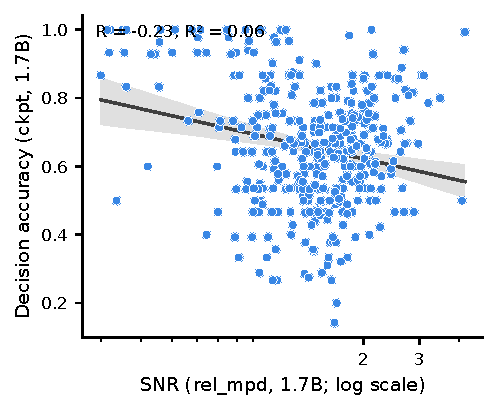
\includegraphics[width=0.5\textwidth]{figures/fig2_snr_vs_da.pdf}
\caption{SNR against decision accuracy by checkpoint at the 1B target, one
point per above-random benchmark, colored by language. Higher SNR predicts
higher decision accuracy.
}
\label{fig:snr-da}
\end{figure}

%\textbf{Language-dependent metric.} The same benchmark may be reliable for some languages and noisy for others. We therefore report all SNR and decision accuracy values per language and aggregate into a benchmark reliability map that practitioners can consult for the languages they target.

\subsection{Framework Generalization}
\label{subsec:exp-generalization}

\textbf{Generalization across seeds.} We test whether the variant ranking survives a change of training seed in our custom pretrained moddels by fitting on two seeds and holding out the third. The variant ranking transfers under DA by checkpoint, with a holdout Spearman correlation of 0.81, and does not transfer under DA by size, with a Spearman correlation of -0.07. The DA-size correlations are small and clustered within roughly 0.1 of each other, so their ranking is noise dominated. The exact best variant per language never transfers either. We therefore recommend a metric family rather than a single variant, and we treat DA-by-size variant rankings as unreliable at this scale.

\textbf{Agreement with the English SNR framework.} We compare our SNR values against those of \citet{heineman_signal_2025} on the DataDecide corpus. Seven English benchmarks are shared between the two model suites, of which four survive the above-random gate. Over these four tasks, SNR values computed on our custom models and on DataDecide agree closely, with a Pearson correlation of 0.98 on log SNR and a Spearman rank correlation of 1.00 under the \texttt{dispersion\_shifted} variant. With so few shared tasks, this is indicative rather than conclusive, but it suggests the framework measures a property of the benchmark rather than of the model suite. % A caveat applies to MMLU, since our suite runs the Cohere translation of the English split while DataDecide runs the original, so this row is not strictly like for like. We plan to rerun the original MMLU task on our checkpoints to remove the alias.

TODO: We will compare our benchmark selection and its compute cost against FineTasks \citep{kydlicek_finetasks_nodate} and SMART filtering \citep{gupta_improving_2025}.


\subsection{Improvement of Benchmark Quality}
\label{subsec:exp-benchmark-design}

%\textbf{Subsampling methods.} We explore subsampling rules that increase SNR on existing benchmarks, including selecting harder questions and removing semantically similar items. The output is a set of higher-SNR subsets that practitioners can use as replacements for full benchmark runs when running ablations. 

\textbf{Benchmarks subtasks are redundant.} Per benchmark, we rank
subtasks by standalone SNR and sweep cumulative subsets
(Figure~\ref{fig:subsets}). A subset of one to two MMLU subjects matches or beats the full set of roughly 48 subjects across model sizes, raising SNR from 2.12 to 3.65 at 175M, and the same subjects recur across sizes and languages. We do not read this as a recommendation to evaluate on a handful of subjects. We read it as evidence that a large share of benchmark content adds variance without adding discriminative signal, so the size of a benchmark is a poor proxy for its reliability. This invites a closer look at which portions of standard suites are informative and which are redundant.

\begin{figure}[t]
\centering
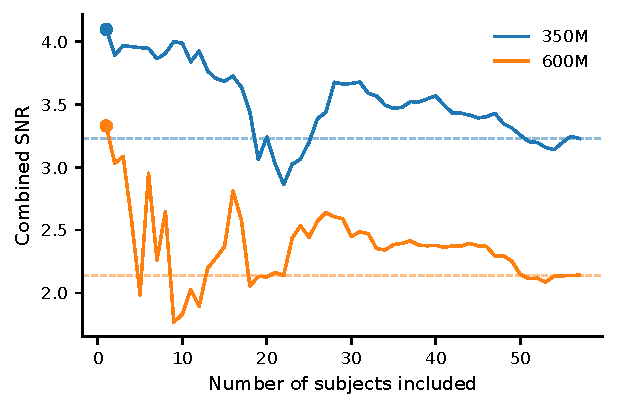
\includegraphics[width=0.6\textwidth]{figures/fig4_subset_sweep.pdf}
\caption{Cumulative subset sweep for Global MMLU subjects. Combined SNR as
subjects are added in order of standalone SNR, one line per model size, with
the full-set SNR as horizontal dashed lines. Small subsets match or beat the
full set.
% TODO: confirm best_n per size from regenerated figure. 
Per-item selection yields larger gains
that do not transfer across sizes.}
\label{fig:subsets}
\end{figure}

\textbf{Item-level subsets.} The same procedure at the level of individual items finds subsets with even larger SNR gains, showing that informative items exist and can be identified within a single model size. The selected items, however, differ across model sizes, with a Jaccard overlap of 0.03 between the best subsets at different scales. Item-level selection is therefore promising as a per-scale tool, and making the selected subsets transfer across scales is the main open problem, which we continue to investigate.

TODO: We will pursue item-level subset selection that transfers across scales, combining our SNR ranking with item response theory approaches \citep{zhou_lost_2026}.


\textbf{Benchmark creation decisions.} We document the data source and curation method of each benchmark in our suite, and compute the correlation between these characteristics and SNR. We classify the data source as web data, news, literature, crowdsourced, expert-generated, or synthetic, and the curation method by whether the data was machine or manually translated and by the review process applied.
We test whether benchmark design features predict SNR on the external suite, where eleven benchmark families clear the above-random gate, including four-option knowledge tasks that capable models solve. No single feature is significant. Family-level Kruskal-Wallis tests on curation method ($p = 0.49$), task format ($p = 1.00$), answer-option count ($p = 0.83$), and source origin ($p = 0.68$) are all far from significance. How a benchmark was built does not predict its reliability once models clear chance on it. The pattern that does hold sits in the answer space, since every benchmark that fails the gate on small models is a four-option translated knowledge task, and benchmarks are sharper when the model compares fewer and longer scored completions. This suggests that for small-scale evaluation, reducing the answer space matters more than curation quality.
